\subsection{Join $\Join$}

\url{https://en.wikipedia.org/wiki/Join_(SQL)#Cross_join}\\

Kombinerer tabeller i en relationel database. Returnere \textit{Cartesian Product}.\\
Vi har tabellen vist på figur~\ref{fig:employee_dept} og tilsvarende vises bruges af Join på listing~\ref{code:crossjoin}.

\begin{figure}[H]
\centering
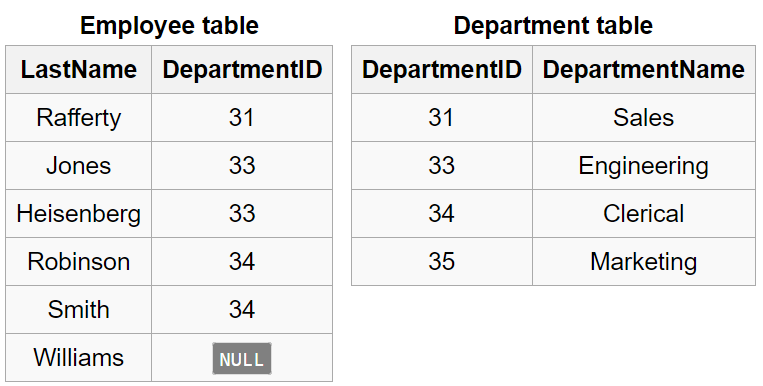
\includegraphics[width=0.6\linewidth]{figs/spm6/employee_dept}
\caption{Eksempel til Join.}
\label{fig:employee_dept}
\end{figure}

Gældende notation ses herunder:

\begin{equation*}
Employee~JOIN_{join~betingelse} Department
\end{equation*}

\begin{lstlisting}[caption=SQL for Cross Join,label=code:crossjoin,morekeywords={SELECT, FROM, WHERE, CROSS, JOIN}]
// Example of an explicit cross join:
SELECT * FROM employee CROSS JOIN department;

// Example of an implicit cross join:
SELECT * FROM employee, department;
\end{lstlisting}

Hvilket returnere en tabel med samtlige kombinationsmuligheder, er tilsvarende eksempel kan ses på figur~\ref{fig:cartesian_product}.

\subsubsection{Cartesian Product*}
Binær operator. Også kaldet \textit{Cross Product} eller \textit{Cross Join}. 

Kombinere tupler i en relation med alle tupler i en anden relation.\\

Som det også kan ses i figur~\ref{fig:cartesian_product} så får hver attribut/kolonne i relation R sin \textit{egen udgave} af hver attribut/kolonne i relation S.

\begin{figure}[H]
	\centering
	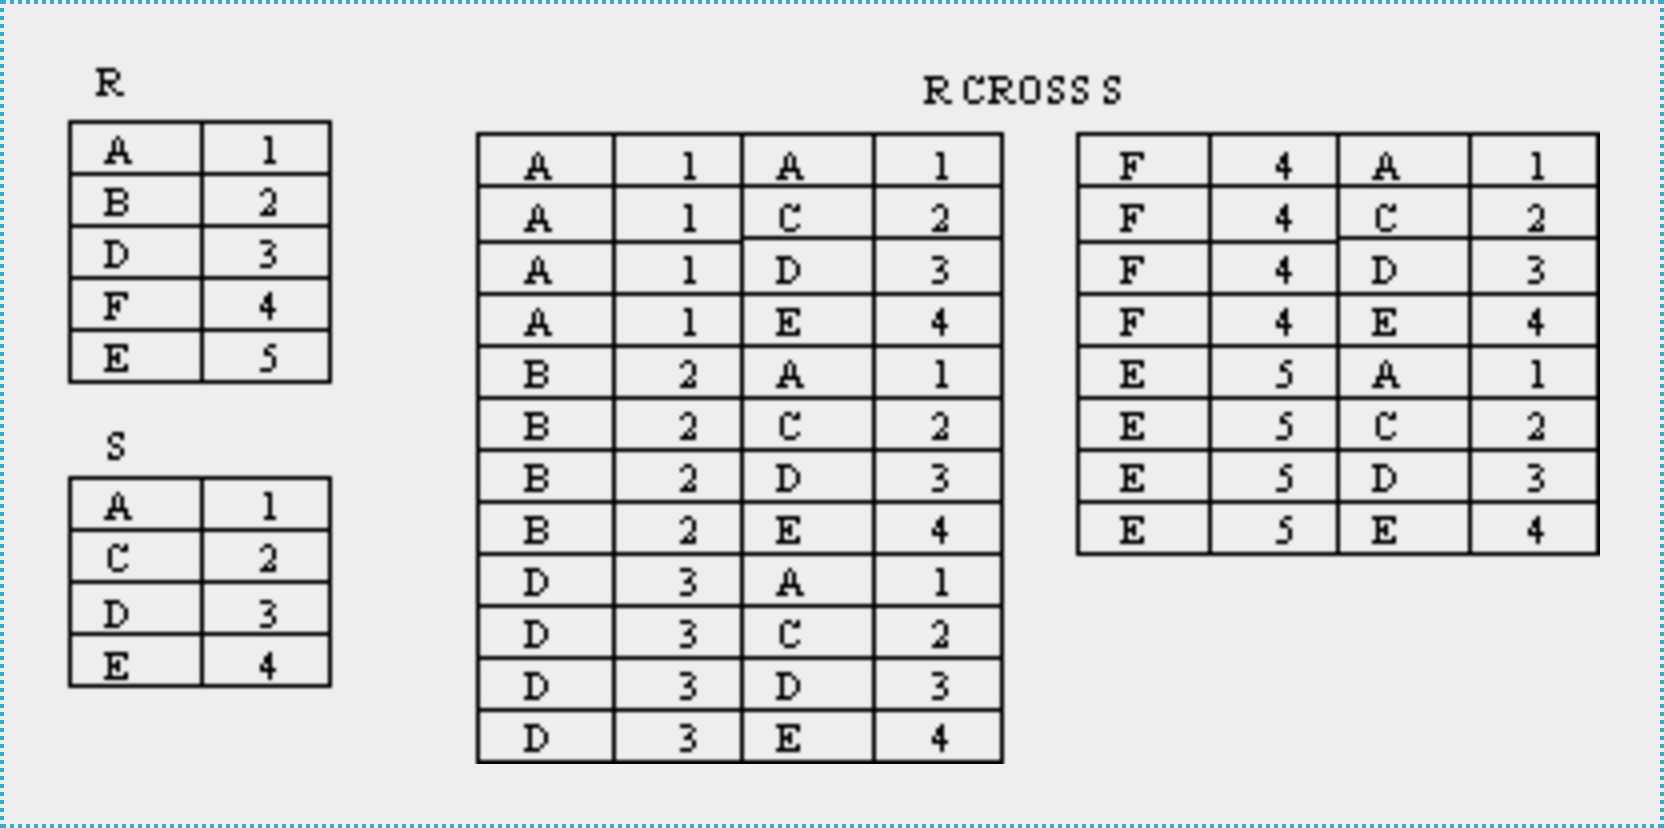
\includegraphics[width=0.7\linewidth]{figs/spm6/cartesianproduct}
	\caption{Eksempel på \textit{cartesian product}.}
	\label{fig:cartesian_product}
\end{figure}

\subsubsection{Right/Left/Full outer Join}

\url{http://db.grussell.org/section010.html#_Toc67114475}\\

\begin{itemize}
	\item \textbf{LEFT OUTER JOIN}\\
	Beholder data fra den venstre tabel. Resten udfyldes med \textit{null}s.
	\item \textbf{RIGHT OUTER JOIN}\\
	Beholder data fra den højre tabel. Resten udfyldes med \textit{null}s.
	\item \textbf{FULL OUTER JOIN}\\
	Beholder data fra begge tabeller (vist på næste side).
\end{itemize}

\begin{figure}[H]
\centering
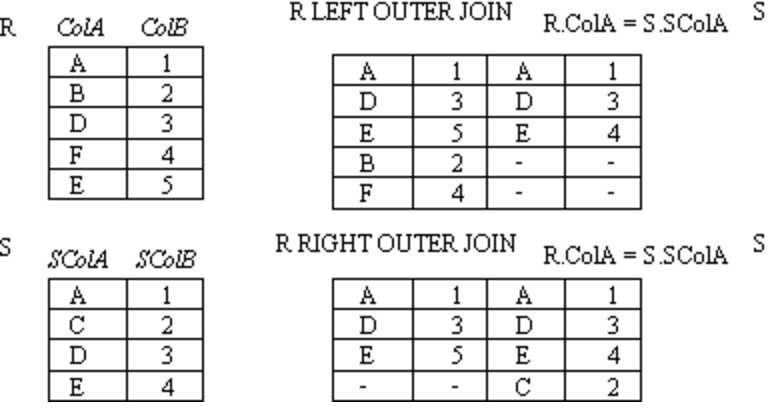
\includegraphics[width=0.6\linewidth]{figs/spm6/outerjoins}
\caption{Eksempel på left-join (øverst) og right-join (nederst).}
\label{fig:outerjoins}
\end{figure}

\begin{lstlisting}[caption=SQL for Left Outer Join,label=code:crossjoin,morekeywords={SELECT, FROM, WHERE, CROSS, JOIN, LEFT, OUTER, ON}]
// Example of an left outer join:
SELECT *
FROM table1
LEFT OUTER JOIN table2
ON table1.column_name = table2.column_name;
\end{lstlisting}

\begin{figure}[H]
\centering
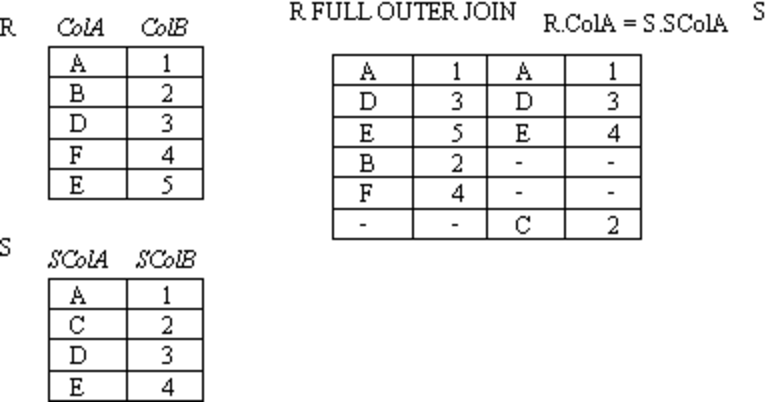
\includegraphics[width=0.6\linewidth]{figs/spm6/fullouterjoin}
\caption{Eksempel på full-outer-join.}
\label{fig:fullouterjoin}
\end{figure}

\subsubsection{Natural Join $\Join$*}

\textit{''The result of the natural join is the set of all combinations of tuples in R and S that are equal on their common attribute names. For an example consider the tables Employee and Dept and their natural join:''}

Det er vigtigt at der ikke er to tabeller med ens navne da \textit{Natural Join} bruger navnet til at finde de attributter som den skal \textit{joine} på.

\begin{figure}[H]
	\centering
	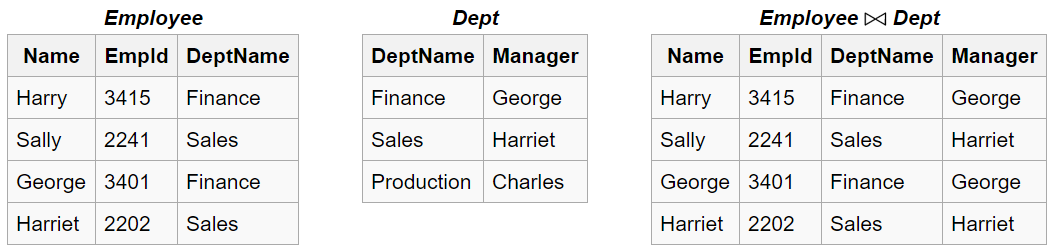
\includegraphics[width=\linewidth]{figs/spm6/naturaljoin}
	\caption{Natural Join illustreret.}
	\label{fig:naturaljoin}
\end{figure}

\begin{lstlisting}[caption=SQL for Cross Join,label=code:crossjoin,morekeywords={SELECT, FROM, WHERE, CROSS, JOIN, NATURAL}]
SELECT * FROM employee NATURAL JOIN department;
\end{lstlisting} 